\section{ Evaluation and Validation}\label{sec:acc_eval}


a mention on differences in measuring accuracy for single-label vs multi
label classifier

mention any metrics that we do not use but are standard, and explain
why we do not use them.

\subsection{Validation Strategy and Sample Space}
In effort to reduce sensitivity to chance selection of random samples, all
measurements are performed using a multi-run stratified 10-fold cross validation.
This gives us a 90/10 train/test data split, and is repeated with a new random
sample shuffling 10 times.
Stratification ensures that there exists an equal class balance in the testing
and training splits.

For each fold, only features from the selected training samples are
used for training and validation.

A total of 3 batches have been computed and merged, giving 12 species in total.
Selection was performed using the mechanisms outlined in
Section~\ref{sec:sample_select}.
Table~\ref{tbl:used_data} shows the selection of species including spectrogram
and template counts per species.

\begin{table}[!htb]
  \caption{Selected species with spectrogram and template counts}
  \label{tbl:used_data}
  \centering
  \begin{tabular}{l r r}
    Species Label & Spectrograms & Templates \\ \hline
    Common Blackbird           & 20 & 6132\\
    Great Reed Warbler         & 20 & 5111\\
    Common Rosefinch           & 20 & 3191\\
    Common Cuckoo              & 20 & 2909\\
    Common Chiffchaff          & 20 & 2886\\
    European Greenfinch        & 20 & 2759\\
    Pale-breasted Spinetail    & 20 & 2501\\
    Ortolan Bunting            & 20 & 2362\\
    Common Reed Bunting        & 20 & 2233\\
    Chestnut-breasted Wren     & 20 & 2203\\
    Corn Bunting               & 20 & 2082\\
    Rufous-browed Peppershrike & 20 & 1404
  \end{tabular}
\end{table}

\subsection{Evaluation Metrics}\label{sec:metrics}
Each of the four evaluation metrics are computed in a fold.
They are then stored and averaged at the end of the 10-fold cross validation.
The four evaluation metrics used are:
\begin{itemize}
  \item \textbf{Accuracy}
    Is the ability of the classifier to correctly label samples.
    \begin{equation}
      \frac{TP+TN}{P+N}
    \end{equation}

  \item \textbf{Precision},
    Sometimes referred to as the positive predictive value, is the ability of the
    classifier to label all predicted values correctly.
    \begin{equation}
      \frac{TP}{TP+FP}
    \end{equation}

  \item \textbf{Recall},
    Sometimes referred to as sensitivity, is the ability of the classifier to
    label all positive samples correctly.
    \begin{equation}
      \frac{TP}{P}
    \end{equation}

  \item \textbf{F-beta score}
    Is the weighted harmonic mean of the precision and recall, where
    higher values indicate better performance.
    This makes it simpler to compare the performance of different parameter sets.
    \begin{equation}
      \frac{(1+\beta^2)TP}{(1+\beta^2)TP+\beta^2FN+FP}
    \end{equation}

    We consider precision and recall as equally important, in which case the
    beta value is set to 1:
    \begin{equation}
      \frac{2TP}{2TP+FN+FP}
    \end{equation}
\end{itemize}
\textbf{move equations to app?}
show how we can extract TP/TN etc from multiclass results (cnf matrix) .. in
appendix prob

The Scikit Learn |precision_recall_fscore_support| function was used to compute
these metrics.

Because this is a multi-class classification task, each metric is computed
on a per-label basis, treating the data as a set of binary classification tasks.
To compute scores for the entire classification task, the values are averaged.
For this we use macro averaging, in which the mean of the scores are computed with equal
weighting, for each one of the metrics.
This is appropriate considering we use stratified k-fold, and each
species is considered equally important to all the others.

\textbf{see about possible multilabel w/o averaging}

\subsubsection{Results}
Results are promising, good performance has been achieved using the initial
parameters, and improvements are observed after tuning as is shown in
Table~\ref{tbl:acc_before_after}.

\textbf{update w/ new defaults}
\textbf{wait for gs results... }
\begin{table}[!htb]
  \centering
  \caption{Comparison of accuracies using default and tuned parameters}
  \label{tbl:acc_before_after}
  \begin{threeparttable}
    \begin{tabular}{l r r}
      & \multicolumn{2}{c}{Metric Scores} \\
      Metric    & Default Params. & Tuned Params. \\ \hline
      Accuracy  & 79.5 (7.3) & 0 \\
      F1 Score  & 77.9 (8.1) & 0 \\
      Recall    & 79.5 (7.4) & 0 \\
      Precision & 82.3 (8.5) & 0
    \end{tabular}
    \begin{tablenotes}
      \footnotesize
      \item[*] Values are shown as percentages.
      \item[*] Standard deviations are shown in parentheses.
    \end{tablenotes}
  \end{threeparttable}
\end{table}

\subsection{AUC curve}
Not yet measured, can use one v one or one v all to measure individual AUC
and then volume under roc hypersurface (vus)
can also compute individual auc for each class if we do try ensembled binary RF

\subsection{Confusion Matrix}
A confusion matrix plots the rate at which each label is predicted as any other
label, where the rows represent the true label, and columns represent the
classifier's predictions.

We construct a confusion matrix to evaluate the performance of the classifier
and the features used to discriminate between species.
In this case the matrix allows us to visualise performance per class, and give
some insight into how the classifier is responding to the selected features.

Figure~\ref{fig:cnf12} shows the resulting confusion matrix from classifying the
selected data, averaged over the 10-run 10-fold cross validation.

\begin{figure}[!htb]
  \centering
  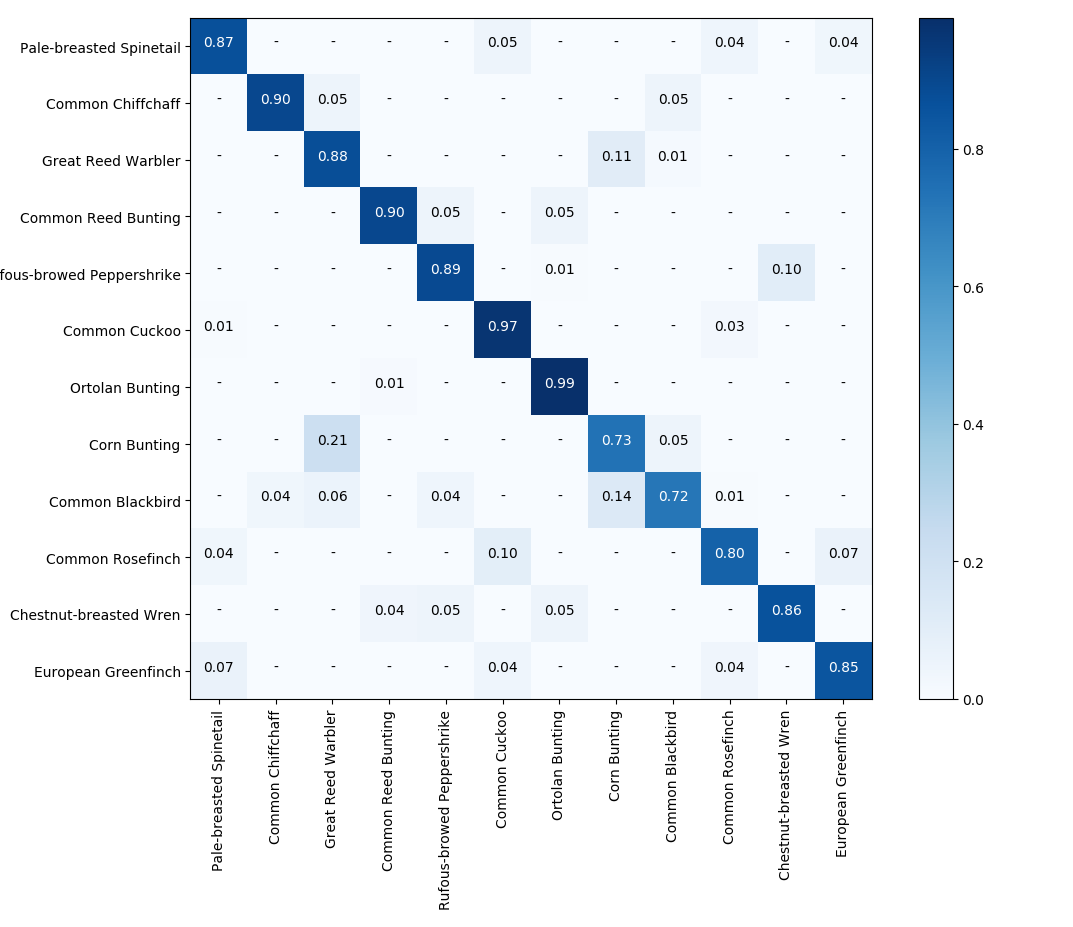
\includegraphics[width=1.0\textwidth]{cnf_matrix_12}
  \caption{Normalized Confusion Matrix}\label{fig:cnf12}
\end{figure}

The confusion matrix shows good classification performance for most species.\\

We can see from the results that the Common Blackbird is the worst performing
classification with a 40\% false negative rate.
It is often mistaken for a Great Reed Warbler, but not the other way around,
which may indicate weakness in the Common Blackbird's templates.

... more speculation

Aside from computing the metrics shown in Section~\ref{sec:metrics}, a confusion
matrix can only offer a speculative insight into template performance.
Nonetheless, it offers a starting point into further template analysis as
discussed in Section~\ref{sec:template_analysis}.
